% PNAS VERSION -- CURRENT WORKING VERSION

\documentclass[9pt,twocolumn,twoside,lineno]{pnas-new}
% Use the lineno option to display guide line numbers if required.

\templatetype{pnasresearcharticle} % Choose template 
% {pnasresearcharticle} = Template for a two-column research article
% {pnasmathematics} %= Template for a one-column mathematics article
% {pnasinvited} %= Template for a PNAS invited submission

\title{Schools are not islands: Balancing COVID-19 risk and educational benefits using structural and temporal countermeasures}

% Use letters for affiliations, numbers to show equal authorship (if applicable) and to indicate the corresponding author
\author[a]{Jamie A. Cohen}
\author[a]{Dina Mistry}
\author[a]{Cliff C. Kerr}
\author[a,1]{Daniel J. Klein}

\affil[a]{Institute for Disease Modeling, Seattle, WA 98109, USA}

% Please give the surname of the lead author for the running footer
\leadauthor{Klein}

% Please add a significance statement to explain the relevance of your work
\significancestatement{%Authors must submit a 120-word maximum statement about the significance of their research paper written at a level understandable to an undergraduate educated scientist outside their field of speciality. The primary goal of the significance statement is to explain the relevance of the work in broad context to a broad readership. The significance statement appears in the paper itself and is required for all research papers.

School reopening during COVID has been a highly contentious topic, with active debates in both the media and the scientific literature. Few model-based analyses have included sufficient detail to represent the real-world scenarios that policymakers are considering, such as classroom cohorting and creative scheduling. To our knowledge, this is the first modeling study that explores the trade-offs between increased risk of COVID-19 transmission and school days lost, taking into account detailed data on school demographics and contact patterns, a set of classroom countermeasures based on proposed policies, and applies them to range of community transmission levels. We find considerable health risks to students, teachers, and staff, but that these risks can be mitigated using non-pharmaceutical interventions, hybrid scheduling, and a phased-in approach that brings back younger students first.}

% Please include corresponding author, author contribution and author declaration information
\authorcontributions{J.A.C. and D.J.K. designed research; J.A.C., D.M., and C.C.K performed research; D.J.K, J.A.C, D.M, and C.C.K wrote the paper.}

\authordeclaration{The authors declare no competing interest.}

%\equalauthors{\textsuperscript{1}A.O.(Author One) contributed equally to this work with A.T. (Author Two) (remove if not applicable).}
%\correspondingauthor{\textsuperscript{1}To whom correspondence should be addressed. E-mail: author.two\@email.com}
\correspondingauthor{\textsuperscript{1}Corresponding author: \href{mailto:dklein@idmod.org}{dklein@idmod.org}}

% At least three keywords are required at submission. Please provide three to five keywords, separated by the pipe symbol.
\keywords{COVID-19 $|$ School reopening $|$ Agent-based modeling $|$ Disease transmission} 

\begin{abstract}
%Please provide an abstract of no more than 250 words in a single paragraph. Abstracts should explain to the general reader the major contributions of the article. References in the abstract must be cited in full within the abstract itself and cited in the text.
COVID-19 outbreaks in schools, day-cares, and camps around the world have demonstrated that in-person learning could place students, teachers, and the broader community at considerable risk. To mitigate this risk, numerous structural and temporal school-based countermeasures have been proposed. Beyond non-pharmaceutical interventions, these measures include classroom cohorting, rotating/hybrid scheduling, and a phased-in approach that returns younger classes first.  To quantify the potential impact of these countermeasures on health risks and educational benefits to school populations and the broader community, we apply the Covasim agent-based COVID-19 transmission model.  Results show that school-based countermeasures can dramatically reduce school-based transmission risks, but that considerable risks will remain if incidence in the broader community is high. Between 5 and 42\% of schools can expect an infected person on the first day of term, depending on the school type and case incidence rate, 20 and 110 per 100,000 over the past two weeks, respectively.  We quantify the COVID-19 infection rate in teachers/staff and students over the first three months of in-person learning for various countermeasures.  While no scenario is risk-free, we robustly find that the cumulative three-month infection rate can be brought down from 25\% for teachers and staff and 17\% for students to levels near or even below 1\%. These results highlight the actions schools and the broader community must take to minimize risk when reopen schools for in-person learning.
\end{abstract}

\dates{This manuscript was compiled on \today}
\doi{\url{www.pnas.org/cgi/doi/10.1073/pnas.XXXXXXXXXX}}

\begin{document}

\maketitle
\thispagestyle{firststyle}
\ifthenelse{\boolean{shortarticle}}{\ifthenelse{\boolean{singlecolumn}}{\abscontentformatted}{\abscontent}}{}

% If your first paragraph (i.e. with the \dropcap) contains a list environment (quote, quotation, theorem, definition, enumerate, itemize...), the line after the list may have some extra indentation. If this is the case, add \parshape=0 to the end of the list environment.
%\dropcap{T}his PNAS journal template is provided to help you write your work in the correct journal format. Instructions for use are provided below. 

%Note: please start your introduction without including the word ``Introduction'' as a section heading (except for math articles in the Physical Sciences section); this heading is implied in the first paragraphs. 

%\section*{Guide to using this template on Overleaf}

%Please note that whilst this template provides a preview of the typeset manuscript for submission, to help in this preparation, it will not necessarily be the final publication layout. For more detailed information please see the \href{https://www.pnas.org/page/authors/format}{PNAS Information for Authors}.

%If you have a question while using this template on Overleaf, please use the help menu (``?'') on the top bar to search for \href{https://www.overleaf.com/help}{help and tutorials}. You can also \href{https://www.overleaf.com/contact}{contact the Overleaf support team} at any time with specific questions about your manuscript or feedback on the template.

\dropcap{P}rimary and secondary schools around the world closed due to COVID-19 transmission in March and April 2020. A recent observational study \cite{auger_association_2020} estimated that school closures were associated with a 62\% decline in weekly COVID-19 incidence and a 58\% decline in weekly COVID-19 mortality; some modeling studies have also found large impacts of school closures \cite{koo2020interventions, panovska2020determining}. However, several other studies \cite{viner_school_2020, esposito_school_2020, ng2020projected} have estimated that closing schools has only a relatively small impact (e.g., 2--4\% reduction in deaths). 

Attention is now focused on the risks and benefits of reopening schools. In-person learning has educational, social, and physical benefits; schools provide a safe space for educational instruction, support the development of social and emotional skills, and address nutritional needs, especially for families of lower socioeconomic status. For these reasons and more, the American Academy of Pediatrics issued a statement \cite{AAPstatement} on July 10 advocating for bringing students back to the classroom for in-person learning. 

Yet much remains uncertain about the role schools, and school-age students in particular, play in COVID-19 transmission, as well as how effective school-based interventions will be in preventing transmission. While children may be both less susceptible and less likely to develop severe infection, nearly a quarter of teachers are at a greater risk of serious illness if infected with COVID-19 \cite{claxton_how_2020}. In an NPR/Ipsos poll of 505 teachers across the US conducted in July, 77\% of teachers indicated that they are worried about risking their own health in returning to in-person education and 66\% would prefer primarily remote, distance learning \cite{kamenetz_most_2020}.

Much can be learned from the experience of school reopening across Europe and Asia; some countries successfully reopened without a significant increase in COVID-19 cases \cite{heavey2020no}, while others were forced to quickly re-close after outbreaks were observed in multiple schools \cite{couzin-frankel_school_2020, vegas_reopening_2020}. In general, countries that reopened schools tended to do so when the case detection rate over the most recent 14 day period was below 25 per 100,000 -- nearly 10 times lower than the case detection rate in the United States as of August 11 \cite{michaud2020}, with significant heterogeneity both across and within states. Additionally, many of these settings returned younger students in-person first with some degree of staggering the start, stop, and break times within schools.

\section*{Results}
To evaluate the health and educational outcomes associated with various school reopening strategies, we used the Covasim agent-based model of COVID-19 transmission. Specifically we compared behavioral interventions such as mask usage, physical distancing and hand hygiene; case detection interventions, including symptomatic screening, follow-up diagnostic testing and contact tracing; and structural interventions, including classroom cohorting, schedule changes, and combinations of remote and in-person learning.

In-person schooling, even with sufficient countermeasures, poses significant risks to students, teachers, and staff. On the first day of school, 5 -- 42\% of schools would have at least one person arrive at school with active COVID-19 (including all students, teachers, and staff), depending on the COVID case detection rate in the community and the school type (Figure \ref{fig:schools_with_a_case}). These infections may show few symptoms and go undetected, especially if they are in younger children. Symptomatic individuals may be screened and sent home immediately upon arrival. Active COVID-19 infections also may not lead to onward transmission within schools, depending on per-contact infectivity. This highlights the importance of procedures within schools to minimize risk of transmission, detect and isolate cases, and contact and quarantine any known contacts. 

\begin{figure}[t] %tbhp
    \centering
    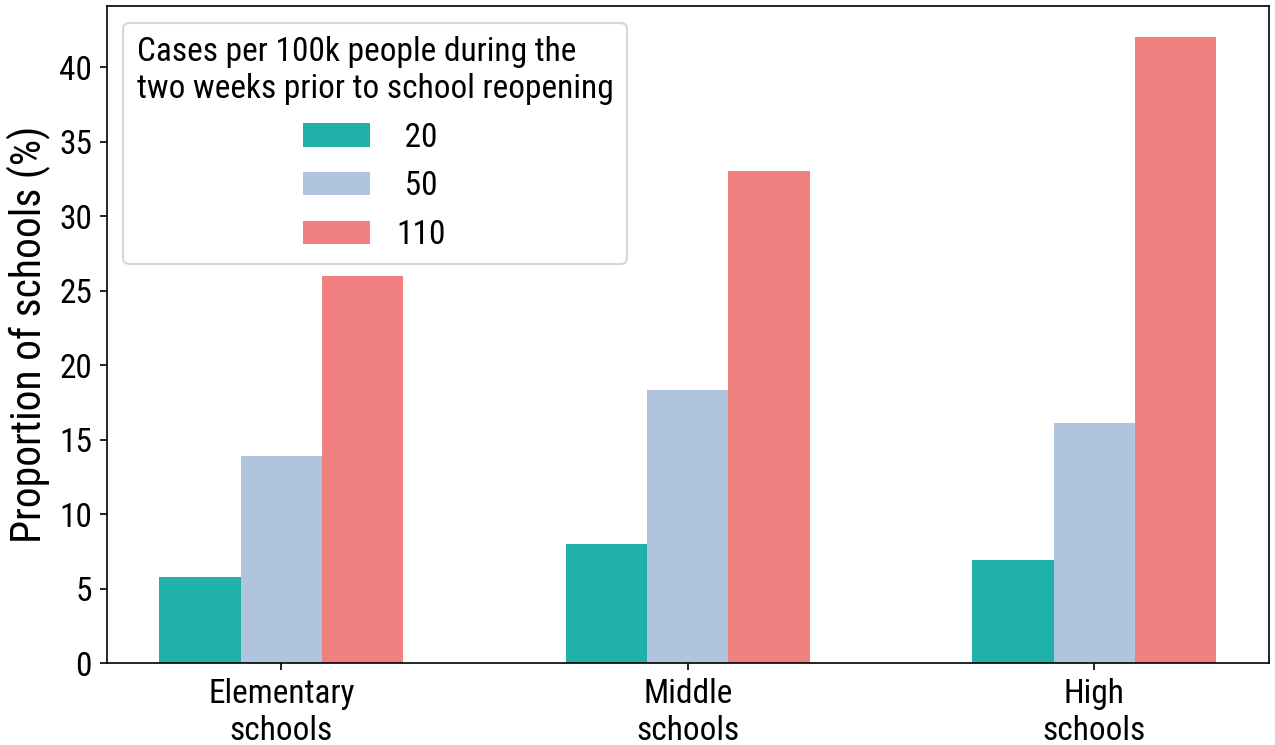
\includegraphics[width=0.9\linewidth]{schools_with_a_case_2020-08-05_trim_notitle.png}
    \caption{Percent of schools with at least one infectious individual arriving on the first day of school. Bars are grouped by school type, with elementary, middle, and high schools covering grades K -- $5$, $6$ -- $8$, and $9$ -- $12$, respectively. Depending on the case incidence rate (bar color), between $5$ and $42\%$ of schools should expect an infectious individual to arrive on the first day of school.}
    \label{fig:schools_with_a_case}
\end{figure}

Closely examining infections present in school, our model shows that in the absence of any countermeasures and at a case detection rate of 110 per 100,000 in the two weeks prior to school reopening, nearly a quarter of teachers and staff and over 17\% of students would visit school while infectious with COVID-19 in the first three months of school (Figure \ref{fig:attack_rate}). This risk can be reduced 2.5-fold by reopening schools when the case detection rate is 20 per 100,000; when there is more COVID in the population, there will inevitably be more COVID in schools. 

We find that implementing countermeasures that limit transmission and detect, trace, and quarantine cases within schools would lead to an even larger reduction in the cumulative COVID-19 infection rate at each of the three case detection rates we considered. The inclusion of face mask usage, physical distancing, classroom cohorting, symptomatic screening, testing and tracing in schools would lower the risk to students, teachers, and staff over 4-fold at a case detection rate of 110 per 100,000. This risk can be lowered further with the addition of scheduling efforts that reduces the number of students present at school. An A/B school scheduling approach that returns elementary schools in-person and keeps all other students remote would minimize the presence of COVID within (and outside of) schools. The predicted cumulative COVID-19 infection rate for people in schools could be as low as between 0.2 and 1.7\% for teachers and staff and to between 0.1 and 1.0\% for students, depending on the case detection rate. This represents at least a 14-fold reduction in the risk of COVID-19 for teachers and staff in schools relative to a strategy that returns all individuals in-person with no countermeasures. Within the King County population of approximately 2.25 million, we estimate that this approach would require an additional 900 -- 6,200 tests for students, teachers and staff over the first three months of school, depending on the case detection rate in the two weeks prior to school.

\begin{figure}[t] %tbhp
    \centering
    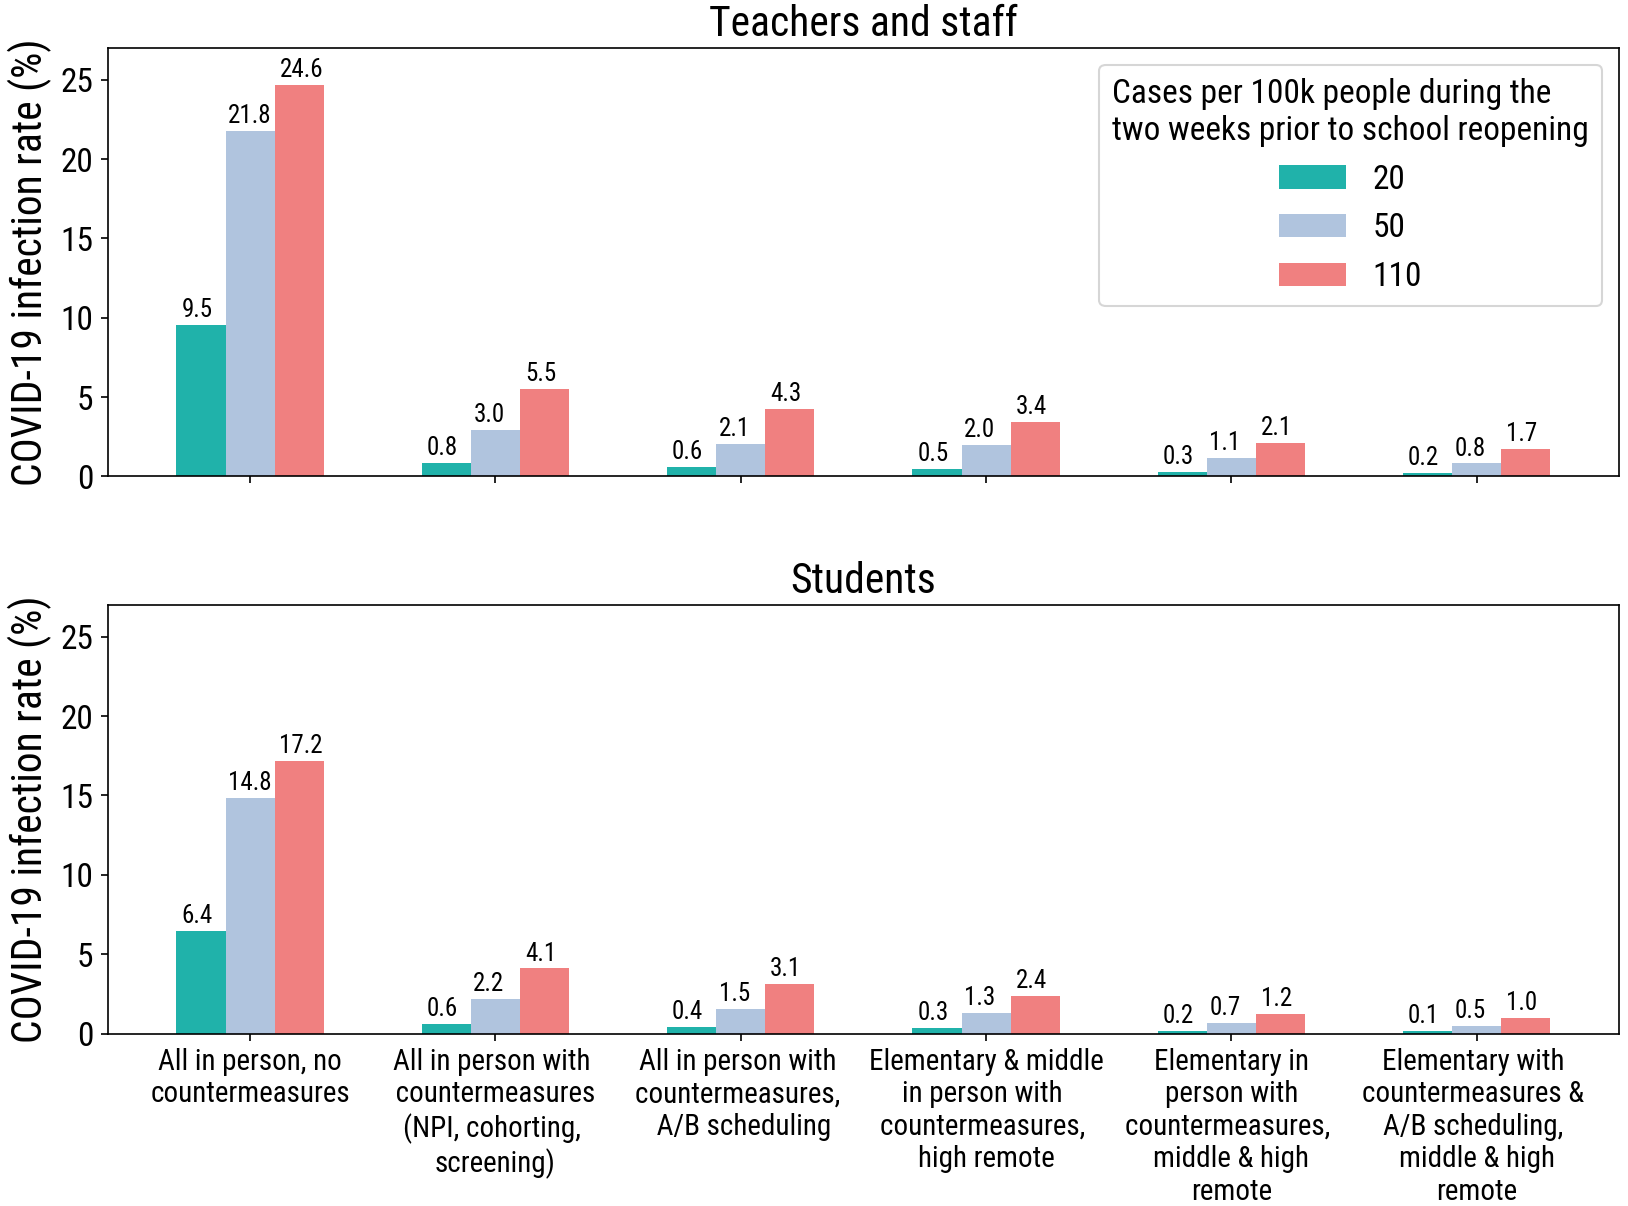
\includegraphics[width=\linewidth]{attack_rate_2020-08-06_trim_notitle.png}
    \caption{Cumulative COVID-19 infection rate for students, teachers and staff physically present in schools during the period of school reopening (Sept 1\textsuperscript{st} - Dec 1\textsuperscript{st}). The attack rate for teachers and staff (top) and for students (bottom) depends on the countermeasures (bar groups) and the case incidence rate in the whole community (bar color).}
    \label{fig:attack_rate}
\end{figure}

We estimate that an A/B scheduling approach, in which classrooms are split into two groups that attend school two days a week on different days, reduces COVID-19 transmission in schools to 0.6 -- 4.3\% for teachers and staff and 0.4 -- 3.1\% for students, depending upon the COVID case detection rate. This represents about double the risk compared to an elementary-only approach, but gives all K-12 students some time for in-person learning, whereas the elementary-only approach restricts in-person learning to elementary school students, at least initially.

These strategies come at a significant educational cost, requiring up to 83\% of school days to be spent at home, due to either planned distance learning or related to detected COVID-19 infection (Figure \ref{fig:tradeoffs}). Provided sufficient countermeasures are implemented within schools, the COVID-19 infection rate in the population prior to school reopening has more influence on the infection rate within schools than the specific schooling strategy.  We find an over seven times reduction in the infection rate for people in schools if schools are reopened when the case detection rate in the community is at 20 per 100,000 compared to 110 per 100,000. At any given case detection rate, additional countermeasures will have a marginal impact on the rate of infection within schools at a large cost of missed in-person school days.

\begin{figure}[t] %tbhp
    \centering
    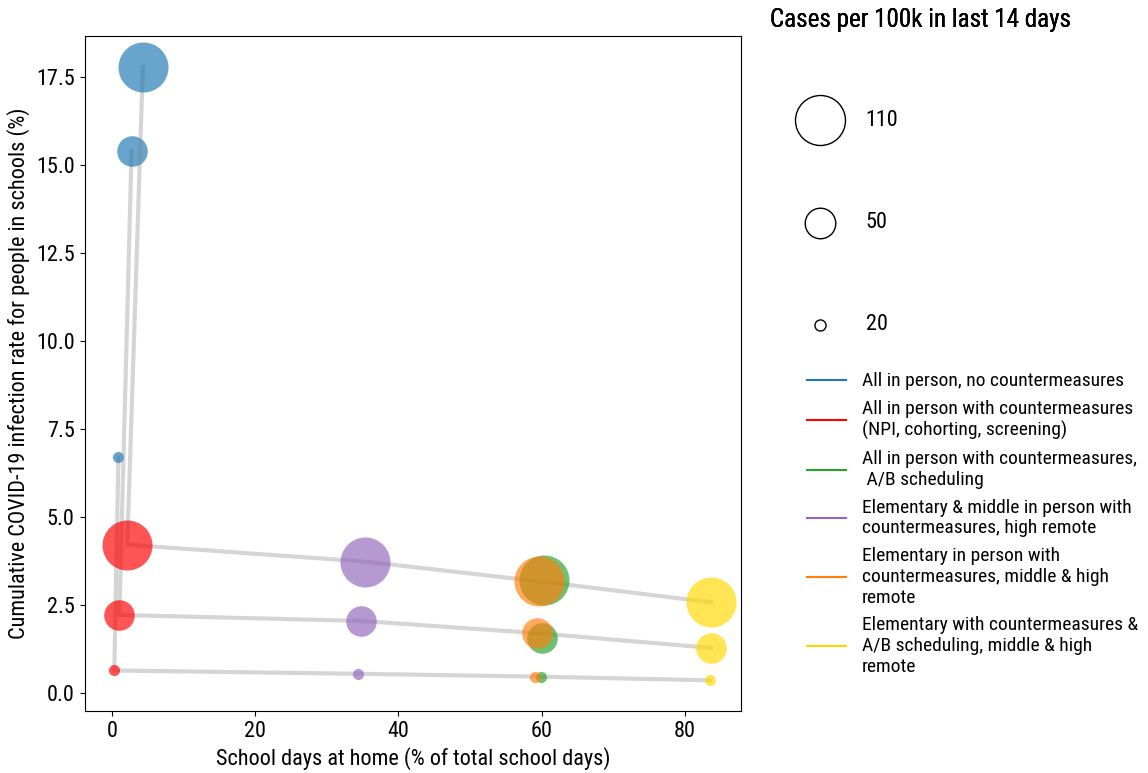
\includegraphics[width=\linewidth]{tradeoffs_2020-08-06_trim_notitle.png}
    \caption{Trade-offs between within-school infection rate and missed in-person school days over the first three months of school reopening. Bubble size corresponds to the case incidence rate in the community over the two weeks prior to school reopening, and gray lines connect the results for each of the three rates considered. The color of each bubble represents the school-based countermeasures. Schools days at home includes quarantine and infection in addition to scheduled distance learning.}
    \label{fig:tradeoffs}
\end{figure}

Reopening schools will not significantly increase community-wide transmission, provided sufficient school-based interventions are implemented (Figure \ref{fig:reff}). If community transmission is decreasing in the absence of in-person schooling, a return to in-person learning with appropriate countermeasures is unlikely to add significantly to community transmission.


\section*{Discussion}

Any return to in-person learning will pose COVID-19 infection risk for students, staff and teachers. However, modeling results suggest that, depending on the case detection rate of COVID-19 in the community, a carefully organized incremental approach that returns the youngest students first with a reduced schedule would minimize the risk of infection within schools and provide important benefits to the neediest children. While this analysis is based upon school enrollment and population demographic data from King County, Washington, lessons can be applied to other settings to inform decision-making around school reopening. For example, as of August 11, 2020, King County had a 14-day case detection rate of 90 compared to 50 in New York City per 100,000 people. This would translate to nearly twice as many schools in the region with at least one person arriving at school with an active COVID-19 infection on September 1\textsuperscript{st} compared to New York City, depending on the size of the school. It may also indicate a different optimal strategy for school reopening in these cities. In fact, Seattle Public Schools, citing a case detection rate in the city of well over 75 per 100,000 in the last two weeks of August, announced they would be starting the fall with completely remote learning \cite{staff_seattle_2020}, while New York Public Schools announced they would start with an A/B hybrid scheduling approach \cite{zaveri_new_2020}. Schools in the San Francisco region have also mostly opted for remote learning, in line with recent model-based recommendations finding a high risk of school reopening \cite{head2020effect}.

We find that the solution with the lowest health risk also has the highest educational cost, in terms of days of distance learning required. We note that days of distance learning are not experienced equally by students and the benefit gained varies considerably based on both age and other factors such as socioeconomic status and resources available to their families \cite{blundell2020covid}. Decision makers must therefore balance the benefits of in-person education with the safety of teachers and staff, while continuing efforts to decrease the incidence of COVID-19 outside of schools. Regardless of the approach taken, it will be critical to monitor schools with symptomatic screening and react quickly to the emergence of cases in schools with testing and contact tracing.

\begin{figure}[t]
    \centering
    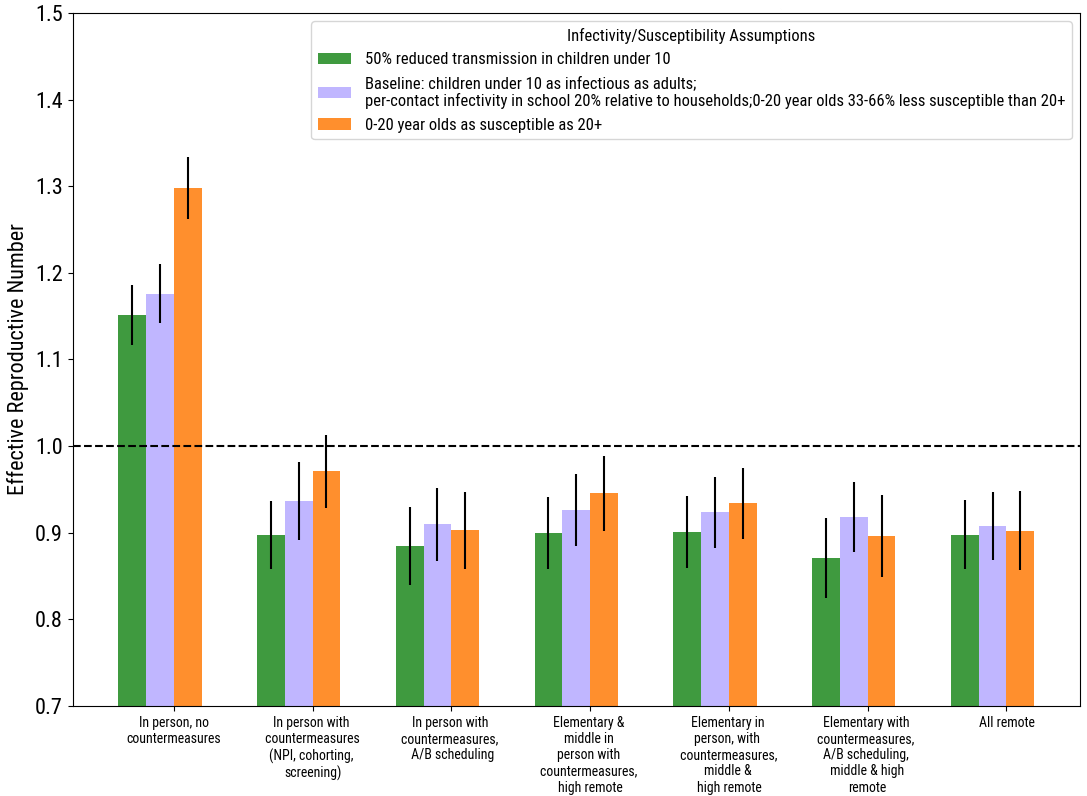
\includegraphics[width=\linewidth]{r_eff_2020-08-13_trim_notitle.png}
    \caption{Effective reproduction number over the simulated period of school reopening (Sept 1\textsuperscript{st} - Dec 1\textsuperscript{st}).  Results are for the COVID-19 case incidence rate of 50 cases per 100,000 in the 14 days prior to school reopening. Results vary with countermeasures (bar groups) and assumptions (bar colors). Error bars represent the standard deviation of the top 20 parameter sets.}
    \label{fig:reff}
\end{figure}

Our results support the strategy of returning elementary school students to school either full-time or with an A/B schedule while keeping all other students remote for the first three months of school to best minimize the risk of COVID-19 infection in schools. Returning elementary schools in-person first is both relatively lower-risk and higher-benefit; elementary school aged children are less susceptible to infection \cite{zhang_changes_2020} and potentially less likely to transmit infection \cite{park_early_nodate, munday2020implications}. Additionally, they may benefit more from in-person learning and pose more of a burden on family members. These results have been put into practice by some countries, which have returned elementary students to school first and older students at a later stage after observing an absence of significant school-based transmission \cite{zhang_changes_2020, auger_association_2020}. However, these countries had a significantly lower COVID-19 incidence rate prior to reopening schools than many parts of the US, including Washington State, are experiencing today.


\subsection*{Limitations}

While agent-based modeling is able to capture many details of populations and disease transmission, our work has important limitations and assumptions that could impact our findings. There is still a high degree of uncertainty around the susceptibility, symptomiticity/severity, and infectivity of COVID-19 in children, particularly since schools in most locations shut down early in the epidemic. Our analysis is based on the most recent scientific literature for each of these parameters. We assumed individuals under 20 had a 45--50\% reduced risk of developing symptoms \cite{davies_age-dependent_nodate} and 33--66\% reduced risk of acquiring infection \cite{zhang_changes_2020}. We varied this in sensitivity analysis so that individuals under 20 are equally as susceptible to infection as individuals age 20 to 50. We assume that an infectious individual is 5 times more likely per day to transmit to a household contact than a school contact, based on estimated numbers of hours spent in each setting per week. We assume all individuals infected with COVID-19 are equally likely to transmit infection per contact, and varied this assumption in sensitivity analysis so that individuals under 10 years old are half as likely.

After being diagnosed, all individuals are assumed to reduce their daily infectivity by 70\% for home contacts, 90\% for community contacts, and 100\% for school and work contacts. Additionally, the household contacts of these individuals may be traced, notified, and school contacts removed from school for a full 14-day quarantine period. While we anticipate that schools will be able to help identify contacts of diagnosed students or staff, the large number of contacts within schools may place additional burden on local or state contact tracing efforts and our analysis does not represent this. We assume that household transmission is not reduced while children are attending school in person, nor that it increases when students are learning remotely.

In terms of structural choices, we made several assumptions about the implementation and impact of school reopening strategies. We chose to not model increased transmission associated with parents/guardians returning to work following a return to in-person learning. We also assume students who participate in remote learning are not in contact with anyone from school. On days that students are learning remotely, we do not account for any potential interaction students may have in a congregate care setting, such as an alternative after-school care program. We have assumed that, if implemented, all elementary and middle schools will be able to enforce classroom cohorting, whereby students are grouped into a classroom and are only in contact with other students and teachers in that classroom. We note that cohorting may be difficult to implement given the complexity of class scheduling for student bodies with multiple academic tracks, elective classes, and degree requirements. Therefore, we may be underestimating the transmission impact of school reopening, and further caution should be taken in any decisions to return to in-person learning.

We assumed that, if implemented, symptomatic screening would occur daily in schools and students or teachers presenting with COVID-like symptoms would be sent home. Those who are symptomatic may be asked to take a diagnostic test, which we assumed returns a result within two days. Students who received a negative test result return to school the next day, and students who received a positive test result are isolated at home for 14 days. Our results do not depend on school staff administering the diagnostic tests. We are not explicitly modeling after-school care, which many working parents depend upon to cover the gap between school hours and working hours. Families who use these services may also be more likely to be essential workers. We also do not model transportation to and from school, which may be an important source of transmission and which also depends on school resources.


\section*{Conclusions}

Schools around the world are grappling with the challenge of returning to in-person learning in the COVID era. Much remains unknown about the role children play in COVID-19 transmission within schools and in the broader community, but the latest science suggests that younger children are less susceptible and show fewer symptoms if infected. From schools that never closed in Sweden to reopening examples in Europe and Asia, lessons on how the US might resume in-person learning are abundant and diverse. Our computational modeling synthesizes this evidence, and the latest results give reason for optimism.

Yet reopening schools is not a zero-risk activity. Symptom screening is imperfect, and COVID-19 will be present in the respiratory system of students, teachers, and staff on day one. Additionally, a return to in-person learning would allow parents and guardians return to work, which could be accompanied by an associated increase in transmission outside schools. But the solution with the lowest health risk has the highest educational cost, the majority of which lands on those families most marginalized and under-resourced: those without access to technology and private tutors, and whose parents or guardians work in the essential economy. Schools must open; the question is when and how, so as to balance the benefits of in-person education with the safety of teachers and staff, all while realizing that COVID is not just a school problem.

%\subsection*{Author Affiliations}

%Include department, institution, and complete address, with the ZIP/postal code, for each author. Use lower case letters to match authors with institutions, as shown in the example. Authors with an ORCID ID may supply this information at submission.

%\subsection*{Submitting Manuscripts}

%All authors must submit their articles at \href{http://www.pnascentral.org/cgi-bin/main.plex}{PNAScentral}. If you are using Overleaf to write your article, you can use the ``Submit to PNAS'' option in the top bar of the editor window. 

%%\subsection*{Format}

%%Many authors find it useful to organize their manuscripts with the following order of sections;  title, author line and affiliations, keywords, abstract, significance statement, introduction, results, discussion, materials and methods, acknowledgments, and references. Other orders and headings are permitted.

%\subsection*{Manuscript Length}

%A standard 6-page article is approximately 4,000 words, 50 references, and 4 medium-size graphical elements (i.e., figures and tables). The preferred length of articles remains at 6 pages, but PNAS will allow articles up to a maximum of 12 pages.

%\subsection*{References}

%References should be cited in numerical order as they appear in text; this will be done automatically via bibtex, e.g. \cite{belkin2002using} and \cite{berard1994embedding,coifman2005geometric}. All references cited in the main text should be included in the main manuscript file.




%\begin{SCfigure*}[\sidecaptionrelwidth][t]
%\centering
%\includegraphics[width=11.4cm,height=11.4cm]{frog}
%\caption{This legend would be placed at the side of the figure, rather than below %it.}\label{fig:side}
%\end{SCfigure*}

%\subsection*{Digital Figures}

%EPS, high-resolution PDF, and PowerPoint are preferred formats for figures that will be used in the main manuscript. Authors may submit PRC or U3D files for 3D images; these must be accompanied by 2D representations in TIFF, EPS, or high-resolution PDF format. Color images must be in RGB (red, green, blue) mode. Include the font files for any text.

%Images must be provided at final size, preferably 1 column width (8.7cm). Figures wider than 1 column should be sized to 11.4cm or 17.8cm wide. Numbers, letters, and symbols should be no smaller than 6 points (2mm) and no larger than 12 points (6mm) after reduction and must be consistent. 

%Figures and tables should be labelled and referenced in the standard way using the \verb|\label{}| and \verb|\ref{}| commands.

%Figure \ref{fig:frog} shows an example of how to insert a column-wide figure. To insert a figure wider than one column, please use the \verb|\begin{figure*}...\end{figure*}| environment. Figures wider than one column should be sized to 11.4 cm or 17.8 cm wide. Use \verb|\begin{SCfigure*}...\end{SCfigure*}| for a wide figure with side legends.

%\subsection*{Tables}
%Tables should be included in the main manuscript file and should not be uploaded separately.

%\subsection*{Single column equations}

%Authors may use 1- or 2-column equations in their article, according to their preference.

%To allow an equation to span both columns, use the \verb|\begin{figure*}...\end{figure*}| environment mentioned above for figures.

%Note that the use of the \verb|widetext| environment for equations is not recommended, and should not be used. 

%\begin{figure*}[bt!]
%\begin{align*}
%(x+y)^3&=(x+y)(x+y)^2\\
%       &=(x+y)(x^2+2xy+y^2) \numberthis \label{eqn:example} \\
%       &=x^3+3x^2y+3xy^3+x^3. 
%\end{align*}
%\end{figure*}


%\begin{table}%[tbhp]
%\centering
%\caption{Comparison of the fitted potential energy surfaces and ab initio benchmark electronic %energy calculations}
%\begin{tabular}{lrrr}
%Species & CBS & CV & G3 \\
%\midrule
%1. Acetaldehyde & 0.0 & 0.0 & 0.0 \\
%2. Vinyl alcohol & 9.1 & 9.6 & 13.5 \\
%3. Hydroxyethylidene & 50.8 & 51.2 & 54.0\\
%\bottomrule
%\end{tabular}

%\addtabletext{nomenclature for the TSs refers to the numbered species in the table.}
%\end{table}

%\subsection*{Supporting Information Appendix (SI)}

%Authors should submit SI as a single separate SI Appendix PDF file, combining all text, figures, tables, movie legends, and SI references. PNAS will publish SI uncomposed, as the authors have provided it. Additional details can be found here: \href{https://www.pnas.org/page/authors/format#Supporting_Information}{policy on SI}. The PNAS Overleaf SI template can be found \href{https://www.overleaf.com/latex/templates/pnas-template-for-supplementary-information/wqfsfqwyjtsd}{here}. Refer to the SI Appendix in the manuscript at an appropriate point in the text. Number supporting figures and tables starting with S1, S2, etc.

%Authors who place detailed materials and methods in an SI Appendix must provide sufficient detail in the main text methods to enable a reader to follow the logic of the procedures and results and also must reference the SI methods. If a paper is fundamentally a study of a new method or technique, then the methods must be described completely in the main text.

%\subsubsection*{SI Datasets} 

%Supply .xlsx, .csv, .txt, .rtf, or .pdf files. This file type will be published in raw format and will not be edited or composed.


%\subsubsection*{SI Movies}

%Supply Audio Video Interleave (avi), Quicktime (mov), Windows Media (wmv), animated GIF (gif), or MPEG files. Movie legends should be included in the SI Appendix file. All movies should be submitted at the desired reproduction size and length. Movies should be no more than 10MB in size.


%\subsubsection*{3D Figures}

%Supply a composable U3D or PRC file so that it may be edited and composed. Authors may submit a PDF file but please note it will be published in raw format and will not be edited or composed.


\matmethods{%Please describe your materials and methods here. This can be more than one paragraph, and may contain subsections and equations as required. Authors should include a statement in the methods section describing how readers will be able to access the data in the paper. 

\subsection*{Model overview}

We used Covasim, an agent-based model of COVID-19 transmission and interventions \cite{kerr_controlling_2020, kerr_covasim_2020}, to estimate the impact of school reopening on disease transmission and the extent to which school-based interventions could mitigate epidemic spread within and outside schools. Covasim includes demographic information on age structure and population size; realistic transmission networks in different social layers, including households, schools, workplaces, long-term care facilities and communities; age-specific disease outcomes; and within- and between-host variations in infectivity to capture sub- and super-spreading and front-loaded infectivity. We modeled schools to match age mixing patterns between students within elementary schools, middle schools, and high schools \cite{guclu_social_2016} (see \hyperref[sec:AppendixA]{Appendix A} for more details on the school network structures). Key inputs and assumptions of our modeling approach have been documented in our methodology papers \cite{kerr_controlling_2020, kerr_covasim_2020}. The Covasim model is fully open source and is available for download via GitHub and the Python Package Index; more information is available at \url{https://covasim.org}.


\subsection*{School reopening scenarios}

We compared seven alternative school reopening strategies that vary the degree of school-based transmission mitigation. Countermeasures were non-pharmaceutical interventions (NPIs), which implicitly include face masks, six foot separation, and hand washing, which together are assumed to reduce transmission by 25\% \cite{chu_physical_2020, lyu_community_2020, chen_hand_2020}; class cohorting, in which students and teachers have minimal contact outside their own classroom (see Figure \ref{fig:school_cohorting}); and symptomatic screening, with 50\% follow-up diagnostic testing and 50\% follow-up contact tracing. A/B scheduling splits classrooms into group A students (who attend two days per week, e.g. Mon-Tue) and group B (who attend two different days per week, e.g. Thu-Fri).

\begin{enumerate}
    \item All in-person with no countermeasures
    \item All in-person with countermeasures
    \item All in-person with countermeasures and A/B scheduling
    \item Elementary and middle in-person with countermeasures, high school remote
    \item Elementary in-person with countermeasures, middle and high school remote
    \item Elementary in-person with countermeasures and A/B scheduling, middle and high school remote
    \item All remote
\end{enumerate}

\begin{figure}[tbhp]
    \centering
    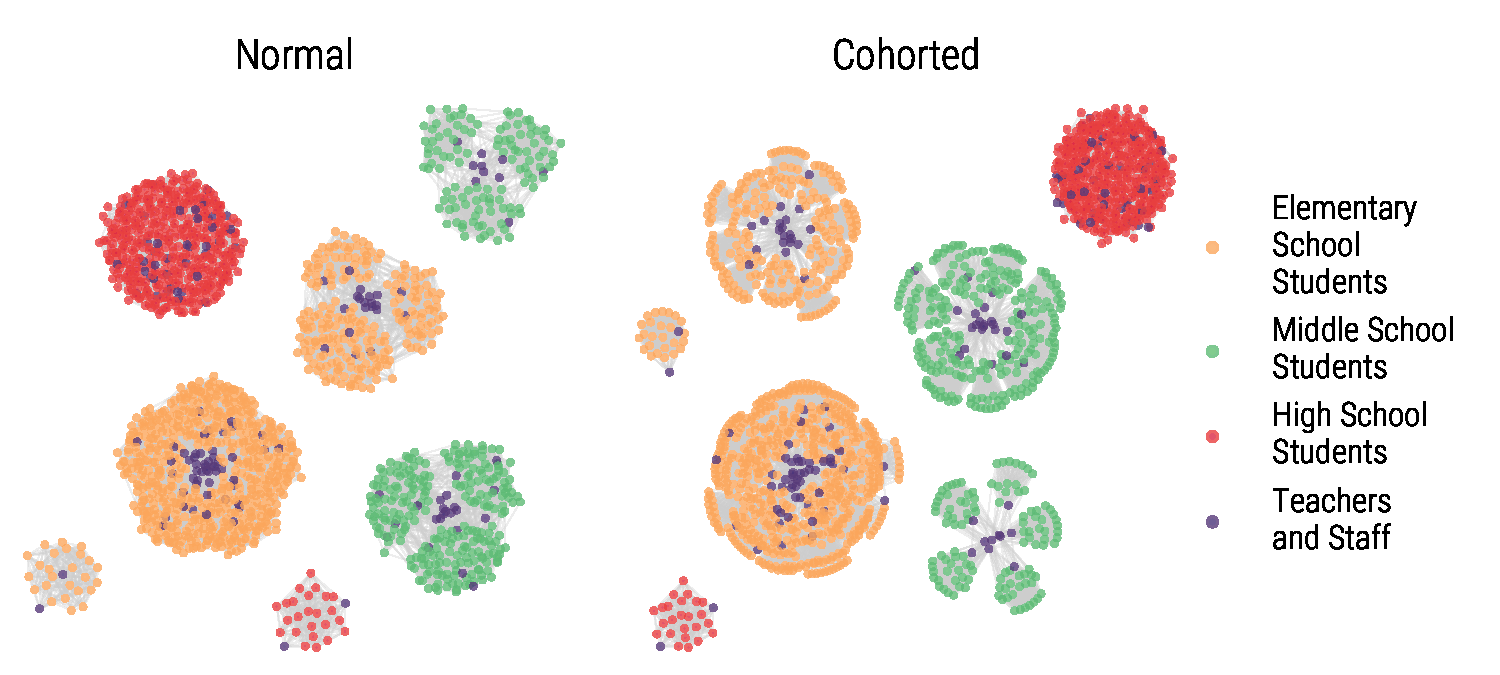
\includegraphics[width=\linewidth]{school_cohorting_1.pdf}
    \caption{A schematic diagram of the in-person school contact networks of students, teachers and additional school staff under different cohorting strategies. Normal, pre-COVID-19 patterns allow for mixing of students and teachers across grades and classrooms. A cohorted strategy places elementary and middle school students into classrooms with their own teachers, preventing contact between students in different classrooms in these schools. High schools remain mixed due to the highly individualized schedules of students in many U.S. based high schools, including those in King County, Washington. Teachers and additional school staff have contacts with each other to reflect their use of common staff paces such as a teachers' lounge, front office, and other rooms for preparation.}
    \label{fig:school_cohorting}
\end{figure}

We applied our interventions to elementary, middle, and high schools and assumed that preschools and universities will remain closed. We assumed that high schools would not be able to implement classroom cohorting, as it would be too challenging to coordinate the highly variable schedules of students at this level (see Figure \ref{fig:school_cohorting} for a schematic of the school network differences). We simulated the first three months of the school term (Sept. 1\textsuperscript{st} - Dec. 1\textsuperscript{st}).

We used data from King County, Washington to define the population and contact network structure, including the average class size and the distribution of students enrolled per school \cite{noauthor_report_nodate}. The effective reproduction number in the absence of school reopening and the case detection rate in the two weeks prior to school reopening served as signals of both the direction of cases as well as the size of the epidemic. Results presented in this work assume that epidemic is declining slowly when schools are fully closed (i.e., $R_e = 0.9$). In conjunction with our assumption around epidemic control with full school closures, we considered three scenarios for the size of the epidemic in the two weeks prior to school reopening: 20, 50, or 110 diagnosed cases per 100,000 individuals. These numbers fit within the low, medium and high case detection bands defined by states across the United States for school re-opening guidance.}

\showmatmethods{} % Display the Materials and Methods section

\acknow{We thank Mike Famulare for early thoughts in shaping this work, and Mandy Izzo and Jen Schripsema for valuable feedback during proof reading.}

\showacknow{} % Display the acknowledgments section

% Bibliography
\bibliography{references}

\end{document}
